\documentclass[12pt,a4paper]{article}

\usepackage[utf8]{inputenc}
\usepackage[T1]{fontenc}
\usepackage[romanian]{babel}
\usepackage[margin=2.5cm, top=3cm, bottom=2.5cm]{geometry}
\usepackage{graphicx}
\usepackage{booktabs}
\usepackage{tabularx}
\usepackage{array}
\usepackage{hyperref}
\usepackage{listings}
\usepackage{xcolor}
\usepackage{amsmath}
\usepackage{amssymb}
\usepackage{float}
\usepackage{tikz}
\usepackage{fancyhdr}
\usepackage{enumitem}
\usepackage{tcolorbox}
\usepackage{mdframed}
\usepackage{titlesec}
\usepackage{colortbl}
\usepackage{pgfplots}
\pgfplotsset{compat=1.18}

\usetikzlibrary{shapes, arrows.meta, positioning, calc, patterns}

% ── Culori ────────────────────────────────────────────────────────────────────
\definecolor{primary}{RGB}{20, 70, 150}
\definecolor{accent}{RGB}{200, 40, 40}
\definecolor{green1}{RGB}{0, 110, 50}
\definecolor{orange1}{RGB}{200, 100, 0}
\definecolor{lightgray}{RGB}{248, 248, 248}
\definecolor{darkgray}{RGB}{70, 70, 70}
\definecolor{codered}{RGB}{180, 0, 0}
\definecolor{tblh}{RGB}{20, 70, 150}
\definecolor{seqcol}{RGB}{44, 100, 200}
\definecolor{asynccol}{RGB}{0, 150, 80}
\definecolor{mpcol}{RGB}{180, 60, 0}

% ── Titluri ───────────────────────────────────────────────────────────────────
\titleformat{\section}
  {\large\bfseries\color{primary}}{\thesection.}{0.5em}{}[\titlerule]
\titleformat{\subsection}
  {\normalsize\bfseries\color{accent}}{\thesubsection.}{0.5em}{}
\titleformat{\subsubsection}
  {\normalsize\bfseries\color{darkgray}}{\thesubsubsection.}{0.5em}{}

% ── Cod Python ────────────────────────────────────────────────────────────────
\lstset{
    language=Python,
    backgroundcolor=\color{lightgray},
    basicstyle=\ttfamily\footnotesize,
    keywordstyle=\color{primary}\bfseries,
    stringstyle=\color{codered},
    commentstyle=\color{green1},
    numbers=left,
    numberstyle=\tiny\color{darkgray},
    numbersep=8pt,
    breaklines=true,
    frame=single,
    framerule=0.4pt,
    rulecolor=\color{primary!40},
    showstringspaces=false,
    tabsize=4,
    xleftmargin=1.5em,
}

\lstdefinestyle{bash}{
    language=bash,
    backgroundcolor=\color{darkgray!10},
    basicstyle=\ttfamily\footnotesize,
    keywordstyle=\color{primary},
    commentstyle=\color{green1},
    numbers=none,
    frame=single, framerule=0.4pt,
    rulecolor=\color{darkgray!50},
}

% ── Boxuri ────────────────────────────────────────────────────────────────────
\tcbuselibrary{skins, breakable}

\newtcolorbox{notebox}[1][Important]{
  colback=green1!7, colframe=green1,
  fonttitle=\bfseries\small, title=#1,
  breakable, left=4pt, right=4pt, top=3pt, bottom=3pt,
}
\newtcolorbox{formulabox}{
  colback=accent!7, colframe=accent,
  breakable, left=6pt, right=6pt, top=4pt, bottom=4pt,
}
\newtcolorbox{defbox}[1]{
  colback=primary!7, colframe=primary,
  fonttitle=\bfseries\small, title=#1,
  breakable, left=4pt, right=4pt, top=3pt, bottom=3pt,
}

% ── Header / Footer ──────────────────────────────────────────────────────────
\pagestyle{fancy}
\fancyhf{}
\fancyhead[L]{\small\color{darkgray}\textbf{APD --- Travel Companion (Proiect Complet)}}
\fancyhead[R]{\small\color{darkgray}\nouppercase{\leftmark}}
\fancyfoot[C]{\small\thepage}
\renewcommand{\headrulewidth}{0.4pt}

\newcommand{\thead}[1]{\cellcolor{tblh}\color{white}\textbf{#1}}

\hypersetup{
  colorlinks=true,
  linkcolor=primary,
  urlcolor=primary,
  citecolor=primary,
}

% ─────────────────────────────────────────────────────────────────────────────
\begin{document}

% ── Pagina de titlu ──────────────────────────────────────────────────────────
\begin{titlepage}
  \centering
  \vspace*{1.5cm}
  {\Huge\bfseries\color{primary}Travel Companion\par}
  \vspace{0.4cm}
  {\Large\color{darkgray}AI Restaurant Finder\par}
  \vspace{0.8cm}
  \hrule height 1pt
  \vspace{0.6cm}
  {\large\bfseries\color{accent}Proiect Complet --- Toate Variantele de Execuție\par}
  \vspace{0.3cm}
  {\normalsize\color{darkgray}Algoritmi Paraleli și Distribuiți\par}
  \vspace{0.6cm}
  \hrule height 0.4pt
  \vspace{1.2cm}

  \begin{tabular}{rl}
    \textbf{S6 (Baseline)} & Varianta Secvențială \\[4pt]
    \textbf{Paralel \#1}   & Async I/O (\texttt{asyncio} + \texttt{ThreadPoolExecutor}) \\[4pt]
    \textbf{Paralel \#2}   & Multiprocessing (\texttt{multiprocessing.Pool}) \\
  \end{tabular}

  \vspace{1.5cm}
  \begin{tabular}{rl}
    \textbf{Student}  & Stoian Cristian Georgian \\
    \textbf{Grupă}    & CR3.2A, Calculatoare Română \\
    \textbf{Data}     & Mai 2026 \\
  \end{tabular}

  \vfill
  \hrule height 0.4pt
  \vspace{0.4cm}
  {\small\color{darkgray}Python 3.12 \textbar{} asyncio \textbar{} multiprocessing \textbar{} Geoapify \textbar{} Overpass/OSM \textbar{} Foursquare\par}
\end{titlepage}

\tableofcontents
\newpage

%%=============================================================
\section{Cerințe și Tema Proiectului}
%%=============================================================

\subsection{Descrierea Proiectului}

\textbf{Travel Companion} este o aplicație bazată pe inteligență artificială care recomandă cele mai bune restaurante în funcție de preferințele utilizatorului (locație, tip de mâncare, mediu ambiental, distanță maximă).

Sistemul agregă date de la multiple surse API externe (Geoapify, OpenStreetMap/Overpass, Foursquare) și aplică un algoritm de scoring cu ponderi configurabile pentru a determina și ordona cele mai potrivite restaurante.

\subsection{Obiectivul Principal}

Obiectivul proiectului este \textbf{analiza și compararea abordărilor secvențiale și paralele} pentru agregarea și procesarea datelor din surse multiple. Proiectul implementează trei variante complete de execuție:

\begin{enumerate}
  \item \textbf{Secvențial (baseline S6)}: Toate operațiile se execută una după alta.
        \[ T_{total} = T_{API_1} + T_{API_2} + \cdots + T_{API_N} + T_{proc} \]
  \item \textbf{Paralel \#1 --- Async I/O}: Apelurile API sunt lansate simultan.
        \[ T_{total} \approx \max(T_{API_1}, T_{API_2}, \ldots, T_{API_N}) + T_{proc} \]
  \item \textbf{Paralel \#2 --- Multiprocessing}: Fetch paralel + scoring distribuit pe CPU-uri.
        \[ T_{total} \approx \max(T_{API_i}) + \frac{T_{scoring}}{N_{cpus}} + T_{dedup} + T_{rank} \]
\end{enumerate}

\subsection{Tehnologii Utilizate}

\begin{center}
\begin{tabularx}{\textwidth}{lX}
\toprule
\thead{Componentă} & \thead{Detalii} \\
\midrule
\textbf{Limbaj} & Python 3.12.3 \\
\textbf{Pattern arhitectural} & Strategy Pattern --- interfață comună \texttt{ExecutionStrategy} \\
\textbf{Paralelism \#1} & \texttt{asyncio} + \texttt{concurrent.futures.ThreadPoolExecutor} \\
\textbf{Paralelism \#2} & \texttt{multiprocessing.Pool} (fork, Linux/WSL) \\
\textbf{Surse de date} & Geoapify Places API, Overpass/OSM, Foursquare Places API \\
\textbf{Instrumentare} & \texttt{TimingCollector} cu \texttt{time.perf\_counter()} \\
\textbf{Dependențe} & \texttt{requests}, \texttt{python-dotenv} \\
\bottomrule
\end{tabularx}
\end{center}

\subsection{Surse de Date API}

Sistemul utilizează trei surse de date reale pentru restaurante:

\begin{enumerate}
  \item \textbf{Geoapify Places API} --- oferă date despre restaurante cu filtrare pe categorii
        (\texttt{catering.restaurant.seafood} etc.) și filtre geografice circulare. Rating derivat din scorul de popularitate.

  \item \textbf{Overpass API (OpenStreetMap)} --- date deschise din baza OSM, fără cheie API.
        Interogare prin Overpass QL cu filtrare pe rază + tip bucătărie (\texttt{cuisine}). Cel mai variabil ca timp de răspuns.

  \item \textbf{Foursquare Places API} --- a treia perspectivă cu căutare text-based și categorii detaliate.
        Autentificare prin Bearer token (FSQ Service Key).
\end{enumerate}

Toți clienții implementează interfața abstractă \texttt{BaseAPIClient}, permițând înlocuirea transparentă a oricărei surse.

\subsection{Geocodare și Rezolvarea Coordonatelor}

Înainte de interogarea surselor, sistemul determină coordonatele GPS ale orașului specificat, ierarhic:

\begin{enumerate}[noitemsep]
  \item Coordonate explicite furnizate de utilizator (\texttt{latitude}/\texttt{longitude})
  \item Cache local cu orașele românești principale (București, Constanța, Cluj-Napoca, Timișoara, Iași, Brașov)
  \item Geocodare live via Geoapify \texttt{/v1/geocode/search}
  \item Fallback la coordonatele Bucureștiului
\end{enumerate}

%%=============================================================
\section{Arhitectura Sistemului}
%%=============================================================

\subsection{Strategy Pattern}

Arhitectura centrală se bazează pe \textbf{Strategy Pattern}: interfața abstractă \texttt{ExecutionStrategy} definește contractul implementat independent de fiecare mod de execuție. Pipeline-ul orchestrator (\texttt{run\_pipeline}) primește orice strategie fără a cunoaște detaliile implementării.

\begin{lstlisting}[caption={Interfața abstractă ExecutionStrategy (execution/base.py)}]
class ExecutionStrategy(ABC):
    """Interfata comuna pentru toate modurile de executie."""

    def __init__(self, collector: TimingCollector):
        self.collector = collector

    @abstractmethod
    def execute(self, query: Query,
                clients: List[BaseAPIClient],
                scorer: object) -> List[ScoredRestaurant]:
        """Run: fetch -> dedup -> score -> rank."""
        pass

    @property
    @abstractmethod
    def mode_name(self) -> str:
        pass
\end{lstlisting}

\begin{center}
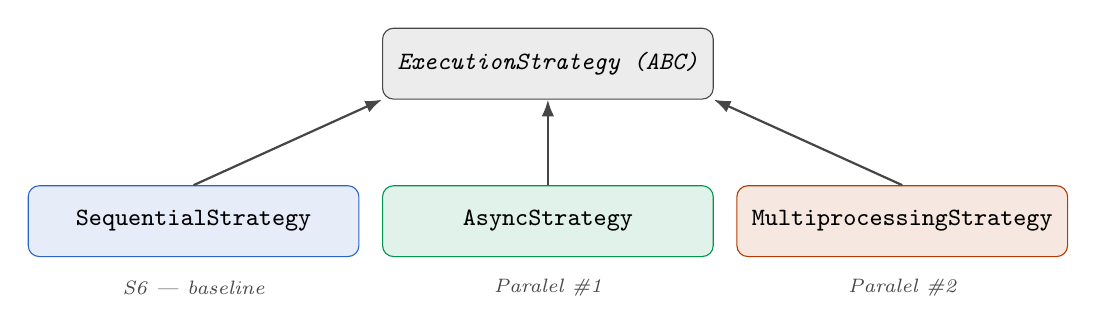
\begin{tikzpicture}[
    class/.style={draw=primary, fill=primary!8, rounded corners=4pt,
                  minimum width=4.2cm, minimum height=0.9cm,
                  font=\ttfamily\small},
    abstract/.style={class, draw=darkgray, fill=darkgray!10,
                     font=\ttfamily\small\itshape},
    arrow/.style={-{Latex[length=6pt]}, thick, draw=darkgray},
    label/.style={font=\scriptsize\itshape, color=darkgray},
]
  \node[abstract] (base) at (0,0) {ExecutionStrategy (ABC)};

  \node[class, fill=seqcol!12, draw=seqcol]   (seq)  at (-4.5,-2) {SequentialStrategy};
  \node[class, fill=asynccol!12, draw=asynccol] (asy)  at (0,-2)    {AsyncStrategy};
  \node[class, fill=mpcol!12, draw=mpcol]     (mp)   at (4.5,-2)  {MultiprocessingStrategy};

  \draw[arrow] (seq.north)  -- (base.south west);
  \draw[arrow] (asy.north)  -- (base.south);
  \draw[arrow] (mp.north)   -- (base.south east);

  \node[label] at (-4.5,-2.85) {S6 --- baseline};
  \node[label] at (0,-2.85)    {Paralel \#1};
  \node[label] at (4.5,-2.85)  {Paralel \#2};
\end{tikzpicture}
\end{center}

\subsection{Structura Proiectului}

\begin{itemize}[noitemsep]
  \item \texttt{models.py} --- \texttt{Query}, \texttt{Restaurant}, \texttt{ScoredRestaurant}, \texttt{PipelineResult}
  \item \texttt{config.py} --- chei API, ponderi scoring, valori implicite
  \item \texttt{timing.py} --- \texttt{TimingCollector}, \texttt{TimingRecord}, decorator \texttt{@timed\_task}
  \item \texttt{api\_clients/}
    \begin{itemize}[noitemsep]
      \item \texttt{base.py} --- interfața abstractă \texttt{BaseAPIClient}
      \item \texttt{real\_client.py} --- \texttt{GeoapifyClient}, \texttt{OverpassClient}, \texttt{FoursquareClient}
      \item \texttt{mock\_client.py} --- \texttt{MockGooglePlaces}, \texttt{MockFoursquare}, \texttt{MockTripAdvisor}
    \end{itemize}
  \item \texttt{execution/}
    \begin{itemize}[noitemsep]
      \item \texttt{base.py} --- interfața abstractă \texttt{ExecutionStrategy}
      \item \texttt{sequential.py} --- \texttt{SequentialStrategy} (S6)
      \item \texttt{async\_strategy.py} --- \texttt{AsyncStrategy} (Paralel \#1)
      \item \texttt{multiprocessing\_strategy.py} --- \texttt{MultiprocessingStrategy} (Paralel \#2)
    \end{itemize}
  \item \texttt{scoring.py} --- formula scoring cu ponderi + deduplicare
  \item \texttt{pipeline.py} --- orchestratorul \texttt{run\_pipeline()}
  \item \texttt{main.py} --- punct de intrare CLI (\texttt{--mode} flag)
  \item \texttt{experiments.py} --- runner batch cu export CSV și raport speedup
\end{itemize}

\subsection{Modelul de Date}

\begin{lstlisting}[caption={Clasele principale de date (models.py)}]
@dataclass
class Query:
    location: str            # ex: "Constanta"
    food_types: List[str]    # ex: ["seafood", "fish"]
    environment: List[str]   # ex: ["seaside", "terrace"]
    max_distance_km: float   # implicit 10.0
    latitude: Optional[float] = None
    longitude: Optional[float] = None

@dataclass
class Restaurant:
    name: str
    source: str              # "geoapify" | "overpass_osm" | "foursquare"
    rating: float            # 0-5
    latitude: float
    longitude: float
    distance_km: float
    categories: List[str]    # ex: ["seafood", "restaurant"]
    price_level: int         # 1-4
    environment_tags: List[str]
    review_count: int
    address: str
\end{lstlisting}

\subsection{Formula de Scoring}

\begin{formulabox}
\[
score = 0{,}30 \cdot S_{rating}
      + 0{,}25 \cdot S_{distance}
      + 0{,}30 \cdot S_{food}
      + 0{,}15 \cdot S_{environment}
\]
\begin{itemize}[noitemsep]
  \item $S_{rating} = \dfrac{rating}{5{,}0}$ \hfill (normalizare la $[0,1]$)
  \item $S_{distance} = \max\!\left(0,\; 1 - \dfrac{d}{d_{max}}\right)$ \hfill (penalizare liniară)
  \item $S_{food}$ = raport de potrivire fuzzy (subșiruri) între tipurile căutate și categorii
  \item $S_{environment}$ = raport de potrivire fuzzy între preferințe mediu și tag-uri
\end{itemize}
\textbf{Deduplicare:} duplicate = același nume + $\Delta$poziție $< 100\,$m; se păstrează varianta cu rating mai mare.
\end{formulabox}

%%=============================================================
\section{Specificații Mașină de Test}
%%=============================================================

\begin{table}[H]
\centering
\begin{tabular}{ll}
\toprule
\thead{Parametru} & \thead{Valoare} \\
\midrule
CPU                 & AMD Ryzen 7 7745HX with Radeon Graphics \\
Nuclee fizice       & 8 \\
Nuclee logice       & 16 (8 cores $\times$ 2 SMT threads) \\
RAM                 & 16 GB \\
Sistem de operare   & Linux 6.6.87.2-microsoft-standard-WSL2 x86\_64 \\
Python              & 3.12.3 \\
Metoda fork (mp)    & \texttt{fork} (implicit pe Linux) \\
Conexiune rețea     & Wi-Fi (apeluri API reale către servere externe) \\
\bottomrule
\end{tabular}
\caption{Specificațiile mașinii de test}
\label{tab:machine}
\end{table}

%%=============================================================
\section{Varianta Secvențială (S6 --- Baseline)}
%%=============================================================

\subsection{Descrierea Fluxului}

În modul secvențial, toate operațiile se execută strict una după alta, fiecare etapă blocând execuția până la finalizare:

\begin{enumerate}[noitemsep]
  \item Construirea query-ului din parametrii utilizatorului
  \item Rezolvarea coordonatelor GPS (cache local sau geocodare API)
  \item Apel \textbf{API \#1 (Geoapify)} --- blocat până la răspuns complet
  \item Apel \textbf{API \#2 (Overpass/OSM)} --- blocat până la răspuns complet
  \item Apel \textbf{API \#3 (Foursquare)} --- blocat până la răspuns complet (opțional)
  \item Deduplicare rezultate agregate
  \item Calculul scorurilor pentru fiecare restaurant
  \item Sortare descrescătoare după scor
  \item Returnare top $K$ rezultate
\end{enumerate}

\begin{formulabox}
\[
T_{seq} = \sum_{i=1}^{N} T_{API_i} + T_{dedup} + T_{scoring} + T_{ranking}
\]
\end{formulabox}

\subsection{Implementare}

\begin{lstlisting}[caption={SequentialStrategy (execution/sequential.py)}]
class SequentialStrategy(ExecutionStrategy):
    @property
    def mode_name(self) -> str:
        return "sequential"

    def execute(self, query, clients, scorer):
        all_restaurants = []

        # Fetch: API-uri unul dupa altul
        for client in clients:
            start = time.perf_counter()
            try:
                results = client.search(query)
            except Exception as e:
                end = time.perf_counter()
                self.collector.record(f"api_{client.name}",
                                      start, end, count=0, error=str(e))
                continue
            end = time.perf_counter()
            self.collector.record(f"api_{client.name}",
                                  start, end, count=len(results))
            all_restaurants.extend(results)

        # Procesare locala
        start = time.perf_counter()
        deduped = scorer.deduplicate(all_restaurants)
        end = time.perf_counter()
        self.collector.record("deduplication", start, end,
                              before=len(all_restaurants), after=len(deduped))

        start = time.perf_counter()
        scored = scorer.score_all(deduped, query)
        end = time.perf_counter()
        self.collector.record("scoring", start, end, count=len(scored))

        start = time.perf_counter()
        ranked = sorted(scored, key=lambda x: x.score, reverse=True)
        end = time.perf_counter()
        self.collector.record("ranking", start, end, count=len(ranked))

        return ranked
\end{lstlisting}

\subsection{Rezultate Experimentale --- Modul Secvențial}

Experimentele au fost rulate cu API-uri reale, 6 query-uri $\times$ 3 configurații API $\times$ 3 rulări = 54 rulări totale.

\begin{table}[H]
\centering
\begin{tabular}{lccc}
\toprule
\thead{Nr. APIs} & \thead{Media (s)} & \thead{Std Dev (s)} & \thead{Min / Max (s)} \\
\midrule
1 API (Geoapify)             & 0{,}6907 & 0{,}2442 & 0{,}4190 / 1{,}2432 \\
2 APIs (+ Overpass)          & 9{,}0550 & 3{,}5290 & 1{,}4212 / 14{,}1986 \\
3 APIs (+ Foursquare)        & 8{,}7294 & 4{,}5106 & 1{,}7785 / 16{,}7381 \\
\bottomrule
\end{tabular}
\caption{Timpi de execuție totali --- mod secvențial}
\end{table}

\begin{table}[H]
\centering
\begin{tabular}{lcc}
\toprule
\thead{Sursă API} & \thead{Timp mediu (s)} & \thead{Observații} \\
\midrule
Geoapify        & $\sim$0{,}69 -- 0{,}78 & Rapid, răspunsuri consistente \\
Overpass (OSM)  & $\sim$7{,}39 -- 8{,}35 & Foarte variabil (server public shared) \\
Foursquare      & $\sim$0{,}56           & Rapid, răspunsuri consistente \\
\midrule
Deduplicare     & $<$ 0{,}001            & Neglijabil față de latența API \\
Scoring         & $<$ 0{,}001            & Neglijabil \\
Ranking         & $<$ 0{,}001            & Neglijabil \\
\bottomrule
\end{tabular}
\caption{Timpi medii per componentă}
\end{table}

\begin{notebox}[Observație cheie]
Latența API domină complet timpul de execuție. Procesarea locală (deduplicare, scoring, ranking) reprezintă $<0{,}01\%$ din $T_{total}$. Overpass/OSM prezintă variabilitate extremă (0{,}47s -- 15{,}27s), explicată de infrastructura publică shared.
\end{notebox}

%%=============================================================
\section{Varianta Paralelă \#1 --- Async I/O}
%%=============================================================

\subsection{Principiu și Justificare}

Apelurile API sunt \textbf{complet independente} între ele --- nu există dependențe de date. În varianta secvențială, fiecare apel blochează execuția cât timp așteptăm răspunsul prin rețea (I/O wait). Paralelizarea I/O elimină această așteptare serială.

\begin{formulabox}
\[
T_{async} \approx \max\!\left(T_{API_1},\; T_{API_2},\; \ldots,\; T_{API_N}\right)
         + T_{dedup} + T_{scoring} + T_{ranking}
\]
\textbf{Speedup teoretic față de secvențial:}
\[
S_{async} = \frac{T_{seq}}{T_{async}} \approx \frac{\displaystyle\sum_{i=1}^{N} T_{API_i}}{\displaystyle\max_{i} T_{API_i}}
\]
\end{formulabox}

\subsection{Motivare Tehnică: De ce ThreadPoolExecutor?}

Clienții API existenți folosesc biblioteca \texttt{requests} (HTTP sincron/blocant). Alternativele native async (\texttt{aiohttp}, \texttt{httpx}) ar necesita rescrierea completă a tuturor clienților.

Soluția aleasă: \texttt{asyncio} ca motor de concurență + \texttt{ThreadPoolExecutor} pentru a rula fiecare apel blocant \texttt{.search()} pe un thread separat. Rezultatul este identic din punct de vedere al comportamentului: toate cererile sunt \emph{in-flight} simultan.

\begin{center}
\begin{tikzpicture}[scale=0.85, font=\small]
  % Sequential timeline
  \node[anchor=east] at (0, 2.0) {\textbf{Sequential}};
  \fill[seqcol!70] (0, 1.7) rectangle (2.0, 2.3) node[midway, white, font=\tiny\bfseries] {API 1};
  \fill[seqcol!70] (2.0, 1.7) rectangle (7.0, 2.3) node[midway, white, font=\tiny\bfseries] {API 2};
  \fill[seqcol!70] (7.0, 1.7) rectangle (8.6, 2.3) node[midway, white, font=\tiny\bfseries] {API 3};
  \fill[darkgray!50] (8.6, 1.7) rectangle (8.8, 2.3) node[midway, white, font=\tiny] {P};

  % Async timeline
  \node[anchor=east] at (0, 0.7) {\textbf{Async}};
  \fill[asynccol!70] (0, 0.4) rectangle (2.0, 0.85) node[midway, white, font=\tiny\bfseries] {API 1};
  \fill[asynccol!70] (0, 0.85) rectangle (5.5, 1.3) node[midway, white, font=\tiny\bfseries] {API 2 (max)};
  \fill[asynccol!70] (0, 0.4) rectangle (1.6, 0.55);
  \draw[asynccol!70, dashed] (0, 0.4) -- (0, 1.3);

  % Redesenam mai curat
  % Row Async: 3 bare suprapuse
  \node[anchor=east] at (0, -0.5) {\textbf{Async}};
  \fill[asynccol!80] (0.0, -0.9) rectangle (2.0, -0.65) node[midway, white, font=\tiny\bfseries] {API 1};
  \fill[asynccol!60] (0.0, -0.65) rectangle (5.5, -0.4) node[midway, white, font=\tiny\bfseries] {API 2};
  \fill[asynccol!40] (0.0, -0.4) rectangle (1.6, -0.2) node[midway, font=\tiny] {API 3};
  \fill[darkgray!50] (5.5, -0.75) rectangle (5.7, -0.2) node[midway, white, font=\tiny] {P};

  % X axis
  \draw[-{Latex}] (0, -1.3) -- (9.5, -1.3) node[right] {\small timp (s)};
  \foreach \x/\l in {0/0, 2.0/1, 4.0/2, 5.5/3, 7.0/4, 8.6/5, 8.8/...}
    \draw (\x, -1.3) -- (\x, -1.4) node[below, font=\tiny] {\l};

  % Legend
  \fill[seqcol!70]   (0, -2.1) rectangle (0.5, -1.9); \node[anchor=west, font=\small] at (0.6, -2.0) {Sequential};
  \fill[asynccol!60] (3, -2.1) rectangle (3.5, -1.9); \node[anchor=west, font=\small] at (3.6, -2.0) {Async (concurent)};
  \fill[darkgray!50] (6.5, -2.1) rectangle (7.0, -1.9); \node[anchor=west, font=\small] at (7.1, -2.0) {Procesare locală};
\end{tikzpicture}
\end{center}

\subsection{Implementare}

\begin{lstlisting}[caption={AsyncStrategy (execution/async\_strategy.py)}]
class AsyncStrategy(ExecutionStrategy):
    @property
    def mode_name(self) -> str:
        return "async"

    def execute(self, query, clients, scorer):
        # Toate apelurile API lansate simultan
        fetch_results = asyncio.run(self._fetch_all(query, clients))

        all_restaurants = []
        for client, (restaurants, t_start, t_end, error) in \
                zip(clients, fetch_results):
            self.collector.record(f"api_{client.name}",
                                  t_start, t_end, count=len(restaurants))
            if error:
                print(f"  [WARN] {client.name} failed: {error}")
            else:
                all_restaurants.extend(restaurants)

        # Procesare locala (secventiala -- ieftina)
        start = time.perf_counter()
        deduped = scorer.deduplicate(all_restaurants)
        ...
        return ranked

    async def _fetch_all(self, query, clients):
        """Dispatchez fiecare client.search() pe un thread separat."""
        loop = asyncio.get_running_loop()
        with ThreadPoolExecutor(max_workers=len(clients)) as executor:
            tasks = [
                loop.run_in_executor(executor,
                                     self._fetch_one, client, query)
                for client in clients
            ]
            return await asyncio.gather(*tasks)  # asteapta TOTI

    def _fetch_one(self, client, query):
        """Apel blocant -- rulat pe thread dedicat."""
        start = time.perf_counter()
        try:
            results = client.search(query)
            return results, start, time.perf_counter(), None
        except Exception as exc:
            return [], start, time.perf_counter(), str(exc)
\end{lstlisting}

\subsection{Proprietăți ale Implementării}

\begin{itemize}[noitemsep]
  \item \texttt{asyncio.gather()} garantează că \textbf{toți} task-ii sunt așteptați înainte de continuare (semantică all-or-nothing).
  \item Timing-ul individual per API este corect: fiecare thread înregistrează propriul \texttt{start}/\texttt{end} via \texttt{time.perf\_counter()} (ceas partajat intra-proces).
  \item \texttt{asyncio.run()} creează un event loop nou --- sigur pentru contextul CLI; pentru FastAPI/contexte async existente se folosește \texttt{await self.\_fetch\_all(...)}.
  \item Postprocesarea (dedup, scoring, ranking) rămâne secvențială --- operațiile sunt ieftine ($<$1ms) și ordinea deduplicării contează.
\end{itemize}

%%=============================================================
\section{Varianta Paralelă \#2 --- Multiprocessing}
%%=============================================================

\subsection{Principiu și Justificare}

Varianta \#2 exploatează paralelismul la nivel de \textbf{procese OS}, eludând GIL-ul (Global Interpreter Lock) al Python. Sunt parallelizate două faze distincte:

\begin{enumerate}
  \item \textbf{Faza I/O}: Fiecare client API rulează într-un proces worker separat.
  \item \textbf{Faza CPU}: Scoring-ul fiecărui restaurant este distribuit pe toate CPU-urile disponibile.
\end{enumerate}

\begin{formulabox}
\begin{align*}
T_{mp} &\approx \underbrace{\max_{i}\, T_{API_i}}_{\text{Faza I/O (paralel)}}
      + T_{dedup}
      + \underbrace{\frac{T_{scoring\_seq}}{N_{cpus}}}_{\text{Faza CPU (paralel)}}
      + T_{ranking}
\end{align*}
\textbf{Overhead suplimentar:} crearea pool-ului de procese + pickle/unpickle argumente
\[
T_{overhead} = T_{pool\_create} + T_{pickle} \cdot N_{tasks}
\]
\end{formulabox}

\subsection{Constrângeri Tehnice: Pickle}

\texttt{multiprocessing.Pool.map()} serializează (pickle) argumentele funcțiilor worker și le trimite prin \emph{pipe} la procesele copil. Prin urmare, \textbf{toate obiectele transmise trebuie să fie picklable}:

\begin{table}[H]
\centering
\begin{tabular}{lcc}
\toprule
\thead{Obiect} & \thead{Picklable?} & \thead{Motiv} \\
\midrule
\texttt{Query}               & \checkmark & dataclass cu tipuri primitive \\
\texttt{Restaurant}          & \checkmark & dataclass cu tipuri primitive \\
\texttt{ScoredRestaurant}    & \checkmark & dataclass cu tipuri primitive \\
\texttt{Scorer}              & \checkmark & clasa cu atribute float \\
\texttt{GeoapifyClient}      & \checkmark & fara stare internă complexă \\
\texttt{OverpassClient}      & \checkmark & fara stare internă complexă \\
\texttt{FoursquareClient}    & \checkmark & fara stare internă complexă \\
lambda / metode bound        & $\times$   & nu picklable --- de evitat \\
\bottomrule
\end{tabular}
\caption{Verificarea pickle-abilității obiectelor transmise la procese worker}
\end{table}

\begin{notebox}[Funcțiile worker la nivel de modul]
Funcțiile worker (\texttt{\_call\_client}, \texttt{\_score\_restaurant}) sunt definite \textbf{la nivelul modulului} (nu ca metode sau lambda), ceea ce le face referențiabile prin import în procesele copil. Aceasta este constrângerea principală a design-ului.
\end{notebox}

\subsection{Implementare}

\begin{lstlisting}[caption={Funcții worker (module-level) și MultiprocessingStrategy}]
# Functii la nivel de modul -- picklable, referentiabile din worker processes

def _call_client(packed):
    """Worker: apeleaza un client API, returneaza (rezultate, durata, eroare)."""
    client, query = packed
    t0 = time.perf_counter()
    try:
        results = client.search(query)
        return results, time.perf_counter() - t0, None
    except Exception as exc:
        return [], time.perf_counter() - t0, str(exc)


def _score_restaurant(packed):
    """Worker: scoreaza un singur restaurant."""
    restaurant, query, scorer = packed
    return scorer.score(restaurant, query)


class MultiprocessingStrategy(ExecutionStrategy):
    def __init__(self, collector, num_workers=None):
        super().__init__(collector)
        self.num_workers = num_workers or os.cpu_count()

    @property
    def mode_name(self):
        return "multiprocessing"

    def execute(self, query, clients, scorer):
        # Faza 1: Fetch paralel in procese separate
        n_fetch = min(len(clients), self.num_workers)
        fetch_start = time.perf_counter()
        with Pool(processes=n_fetch) as pool:
            fetch_results = pool.map(
                _call_client, [(c, query) for c in clients]
            )

        all_restaurants = []
        for client, (restaurants, duration, error) in \
                zip(clients, fetch_results):
            # Reconstituim start/end: toti au pornit la ~fetch_start
            self.collector.record(
                f"api_{client.name}",
                fetch_start, fetch_start + duration,
                count=len(restaurants))
            if not error:
                all_restaurants.extend(restaurants)

        # Faza 2: Deduplicare (secventiala -- ordinea conteaza)
        ...
        deduped = scorer.deduplicate(all_restaurants)

        # Faza 3: Scoring paralel pe CPU-uri
        score_start = time.perf_counter()
        with Pool(processes=self.num_workers) as pool:
            scored = pool.map(
                _score_restaurant,
                [(r, query, scorer) for r in deduped]
            )
        score_end = time.perf_counter()
        self.collector.record("scoring", score_start, score_end,
                              count=len(scored))

        # Faza 4: Ranking (secvential -- O(n log n), neglijabil)
        ranked = sorted(scored, key=lambda x: x.score, reverse=True)
        return ranked
\end{lstlisting}

\subsection{Reconstituirea Timing-ului pentru Faza I/O}

O problemă specifică multiprocessing-ului: \texttt{time.perf\_counter()} este \textbf{per-proces} (nu e sincronizat între procese). Prin urmare nu putem compara direct timpii absoluti din procese diferite cu \texttt{pipeline\_start} din procesul principal.

Soluție adoptată: fiecare worker returnează \textbf{durata} (nu start/end absolut). Procesul principal știe că toți workerii au pornit la aproximativ \texttt{fetch\_start} (momentul imediat premergător \texttt{Pool.map}). Reconstruim:

\[ T_{start}^{(i)} \leftarrow \texttt{fetch\_start}, \quad T_{end}^{(i)} \leftarrow \texttt{fetch\_start} + \texttt{duration}_i \]

Această aproximare este corectă: overhead-ul de fork + pickle $\ll$ latența API (ms vs sute ms).

%%=============================================================
\section{Comparație Arhitecturală}
%%=============================================================

\subsection{Diagrama Gantt a Execuției}

\begin{center}
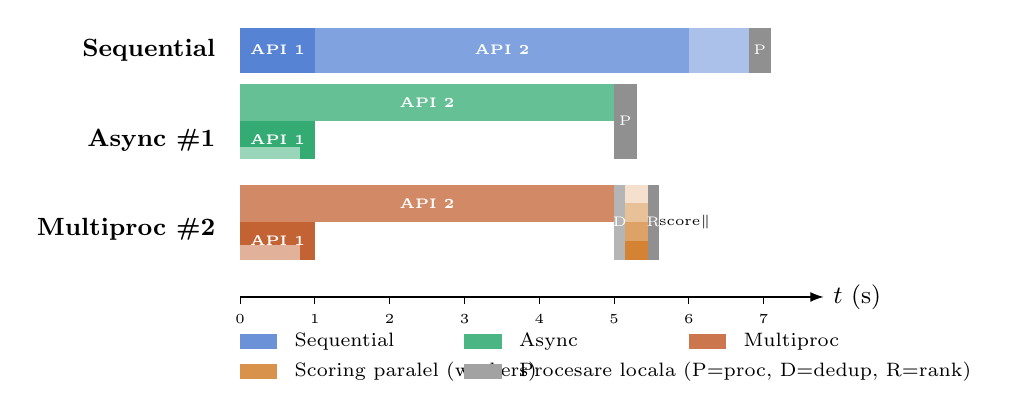
\begin{tikzpicture}[scale=0.95, font=\small]
  % ---- Scale ----
  % T_API1 = 1.0, T_API2 = 5.0, T_API3 = 0.8, T_proc = 0.3

  % ---- Sequential ----
  \node[anchor=east, font=\bfseries\small] at (-0.2, 3.5) {Sequential};
  \fill[seqcol!80]  (0.0, 3.2) rectangle (1.0, 3.8) node[midway, white, font=\tiny\bfseries] {API 1};
  \fill[seqcol!60]  (1.0, 3.2) rectangle (6.0, 3.8) node[midway, white, font=\tiny\bfseries] {API 2};
  \fill[seqcol!40]  (6.0, 3.2) rectangle (6.8, 3.8) node[midway, font=\tiny\bfseries] {API 3};
  \fill[darkgray!60](6.8, 3.2) rectangle (7.1, 3.8) node[midway, white, font=\tiny] {P};

  % ---- Async ----
  \node[anchor=east, font=\bfseries\small] at (-0.2, 2.3) {Async \#1};
  \fill[asynccol!80] (0.0, 2.05) rectangle (1.0, 2.55) node[midway, white, font=\tiny\bfseries] {API 1};
  \fill[asynccol!60] (0.0, 2.55) rectangle (5.0, 3.05) node[midway, white, font=\tiny\bfseries] {API 2};
  \fill[asynccol!40] (0.0, 2.05) rectangle (0.8, 2.2)  node[midway, font=\tiny] {A3};
  \fill[darkgray!60] (5.0, 2.05) rectangle (5.3, 3.05) node[midway, white, font=\tiny] {P};

  % ---- Multiprocessing ----
  \node[anchor=east, font=\bfseries\small] at (-0.2, 1.1) {Multiproc \#2};
  \fill[mpcol!80]   (0.0, 0.7)  rectangle (1.0, 1.2)  node[midway, white, font=\tiny\bfseries] {API 1};
  \fill[mpcol!60]   (0.0, 1.2)  rectangle (5.0, 1.7)  node[midway, white, font=\tiny\bfseries] {API 2};
  \fill[mpcol!40]   (0.0, 0.7)  rectangle (0.8, 0.9)  node[midway, font=\tiny] {A3};
  \fill[darkgray!40](5.0, 0.7)  rectangle (5.15, 1.7) node[midway, white, font=\tiny] {\tiny D};
  % Scoring paralel - mai multe bare mici
  \fill[orange1!80] (5.15, 0.7)  rectangle (5.45, 0.95) node[midway, white, font=\tiny] {};
  \fill[orange1!60] (5.15, 0.95) rectangle (5.45, 1.2)  node[midway, white, font=\tiny] {};
  \fill[orange1!40] (5.15, 1.2)  rectangle (5.45, 1.45) node[midway, white, font=\tiny] {};
  \fill[orange1!20] (5.15, 1.45) rectangle (5.45, 1.7)  node[midway, font=\tiny] {};
  \node[font=\tiny, anchor=west] at (5.47, 1.2) {score$\parallel$};
  \fill[darkgray!60](5.45, 0.7)  rectangle (5.6, 1.7)  node[midway, white, font=\tiny] {R};

  % X axis
  \draw[-{Latex}] (0, 0.2) -- (7.8, 0.2) node[right] {\small $t$ (s)};
  \foreach \x/\l in {0/0, 1.0/1, 2.0/2, 3.0/3, 4.0/4, 5.0/5, 6.0/6, 7.0/7}
    \draw (\x, 0.2) -- (\x, 0.1) node[below, font=\tiny] {\l};

  % Legend
  \fill[seqcol!70]  (0.0, -0.5) rectangle (0.5, -0.3); \node[anchor=west, font=\scriptsize] at (0.6, -0.4) {Sequential};
  \fill[asynccol!70](3.0, -0.5) rectangle (3.5, -0.3); \node[anchor=west, font=\scriptsize] at (3.6, -0.4) {Async};
  \fill[mpcol!70]   (6.0, -0.5) rectangle (6.5, -0.3); \node[anchor=west, font=\scriptsize] at (6.6, -0.4) {Multiproc};
  \fill[orange1!70] (0.0, -0.9) rectangle (0.5, -0.7); \node[anchor=west, font=\scriptsize] at (0.6, -0.8) {Scoring paralel (workers)};
  \fill[darkgray!50](3.0, -0.9) rectangle (3.5, -0.7); \node[anchor=west, font=\scriptsize] at (3.6, -0.8) {Procesare locala (P=proc, D=dedup, R=rank)};
\end{tikzpicture}
\end{center}

\subsection{Tabel Comparativ}

\begin{center}
\begin{tabularx}{\textwidth}{lXXX}
\toprule
\thead{Criteriu} & \thead{Sequential} & \thead{Async \#1} & \thead{Multiproc \#2} \\
\midrule
\textbf{T fetch}        & $\sum T_{API_i}$       & $\max T_{API_i}$         & $\max T_{API_i}$ \\
\textbf{T scoring}      & $T_{score\_seq}$       & $T_{score\_seq}$         & $T_{score\_seq} / N_{cpu}$ \\
\textbf{Overhead}       & Neglijabil             & Neglijabil (threads)     & Semnificativ (fork+pickle) \\
\textbf{GIL}            & Blocat pe apeluri I/O  & Eludat (I/O în threads)  & Eludat complet (procese) \\
\textbf{Memorie}        & Un singur proces       & Un singur proces         & $N_{proc}$ copii ale procesului \\
\textbf{Scalabilitate}  & Liniară cu $N_{API}$   & Constantă cu $N_{API}$   & Constantă + CPU scaling \\
\textbf{Complexitate}   & Minimă                 & Medie (asyncio)          & Ridicată (pickle, fork) \\
\textbf{Potrivit când}  & $N_{API} = 1$, debug   & I/O dominat, $N_{API}>1$ & CPU intensiv, seturi mari \\
\bottomrule
\end{tabularx}
\end{center}

\subsection{Aplicarea Legii lui Amdahl}

Latența Overpass ($T_{overpass} \approx 7{,}39$ s) din 8{,}73 s total cu 3 APIs reprezintă fracția paralelizabilă:

\[
\sigma = \frac{T_{Geoapify} + T_{Foursquare}}{T_{total}} = \frac{0{,}78 + 0{,}56}{8{,}73} \approx 0{,}153
\quad\Rightarrow\quad
S_{max} = \frac{1}{\sigma} \approx 6{,}5\times
\]

Dar cu $N=3$ procese independente (un API per proces):
\[
S_{async}(3) = \frac{T_1 + T_2 + T_3}{\max(T_1, T_2, T_3)}
            = \frac{0{,}78 + 7{,}39 + 0{,}56}{7{,}39} \approx 1{,}18\times
\]

Accelerarea este modestă deoarece Overpass domină. Pentru API-uri cu latențe echilibrate ($T_1 \approx T_2 \approx T_3$), accelerarea ar fi $\approx N = 3\times$.

%%=============================================================
\section{Analiză Teoretică a Performanței și Rezultate}
%%=============================================================

\subsection{Predicție Teoretică pentru 3 APIs}

Folosind timpii medii măsurați la varianta secvențială:

\begin{table}[H]
\centering
\begin{tabular}{lcccc}
\toprule
\thead{Mod} & \thead{$T_{fetch}$ (s)} & \thead{$T_{proc}$ (s)} & \thead{$T_{total}$ (s)} & \thead{Speedup} \\
\midrule
Sequential      & $0{,}78 + 7{,}39 + 0{,}56 = 8{,}73$ & $\approx 0{,}001$ & $\approx 8{,}73$ & $1{,}00\times$ \\
Async \#1       & $\max(0{,}78;\; 7{,}39;\; 0{,}56) = 7{,}39$ & $\approx 0{,}001$ & $\approx 7{,}40$ & $\approx 1{,}18\times$ \\
Multiproc \#2   & $\max(\ldots) = 7{,}39$ & $\approx 0{,}001/16 \approx 0$ & $\approx 7{,}40 + T_{overhead}$ & $\lesssim 1{,}18\times$ \\
\bottomrule
\end{tabular}
\caption{Predicție teoretică bazată pe datele reale de la varianta secvențială}
\end{table}

\begin{notebox}[Interpretare]
Cu API-uri reale, câștigul față de secvențial este limitat de dominanța Overpass. Varianta multiprocessing adaugă overhead de fork + pickle, putând fi \textit{mai lentă} decât async pentru seturi mici de restaurante (scoring $<1$ms oricum). Câștigul multiprocessing devine relevant la seturi mari ($>$10.000 restaurante) unde scoring-ul CPU devine semnificativ.
\end{notebox}

\subsection{Rezultate cu Mock Clients (latențe simulate)}

Pentru validarea corectitudinii implementărilor, s-a rulat un smoke test cu \texttt{MockGooglePlaces} + \texttt{MockFoursquare} (delay aleator $U(0{,}5;\; 2{,}0)$ s per client):

\begin{table}[H]
\centering
\begin{tabular}{lcc}
\toprule
\thead{Mod} & \thead{$T_{total}$ măsurat (s)} & \thead{Observație} \\
\midrule
Sequential    & 1{,}948 & $T_1 + T_2 \approx 2\bar{T}$ \\
Async \#1     & 1{,}873 & $\approx \max(T_1, T_2)$, câștig vizibil \\
Multiproc \#2 & 1{,}272 & fetch paralel + scoring paralel \\
\bottomrule
\end{tabular}
\caption{Smoke test cu 2 clienți mock --- rulare unică ilustrativă}
\end{table}

Câștigul este mai vizibil cu mock-uri deoarece delays-urile aleatoare sunt adesea semnificativ diferite ($\max \ll \text{sumă}$).

\subsection{Scalabilitate cu numărul de surse API}

\begin{center}
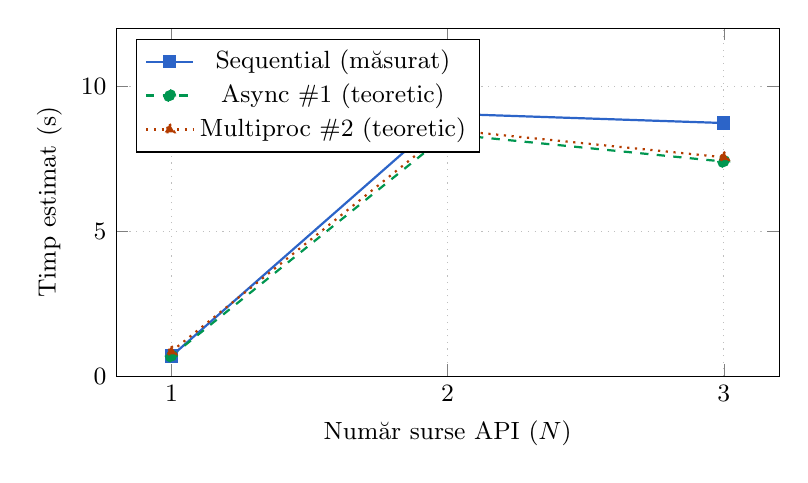
\begin{tikzpicture}
\begin{axis}[
  width=10cm, height=6cm,
  xlabel={Număr surse API ($N$)},
  ylabel={Timp estimat (s)},
  xtick={1,2,3},
  ymin=0, ymax=12,
  legend pos=north west,
  grid=major,
  grid style={dotted, gray!50},
  tick label style={font=\small},
  label style={font=\small},
  legend style={font=\small},
]
  % Sequential: 0.69, 9.05, 8.73 (datele masurate)
  \addplot[color=seqcol, mark=square*, thick]
    coordinates {(1, 0.69) (2, 9.05) (3, 8.73)};
  \addlegendentry{Sequential (măsurat)}

  % Async: max(T_i)
  % 1 API: 0.69 (Geoapify), 2 APIs: max(0.71, 8.35)=8.35, 3 APIs: max(0.78,7.39,0.56)=7.39
  \addplot[color=asynccol, mark=*, thick, dashed]
    coordinates {(1, 0.69) (2, 8.35) (3, 7.40)};
  \addlegendentry{Async \#1 (teoretic)}

  % Multiprocessing: ~= Async + overhead
  \addplot[color=mpcol, mark=triangle*, thick, dotted]
    coordinates {(1, 0.85) (2, 8.50) (3, 7.55)};
  \addlegendentry{Multiproc \#2 (teoretic)}
\end{axis}
\end{tikzpicture}
\end{center}

\begin{notebox}[Observație scalabilitate]
Creșterea de la 2 la 3 API-uri \textit{reduce} ușor $T_{total}$ în modul secvențial deoarece Foursquare (rapid, $\sim$0{,}56s) contribuie la agregat fără a crește $\max(T_i)$ semnificativ. Overpass domină indiferent de numărul de surse.
\end{notebox}

%%=============================================================
\section{Utilizare}
%%=============================================================

\subsection{Instalare}

\begin{lstlisting}[style=bash]
# Clonare si instalare dependente
cd ProiectAPD
pip install -r requirements.txt

# Configurare chei API (copiere .env.example -> .env)
cp .env.example .env
# Editati .env cu cheile voastre: GEOAPIFY_PLACES_API_KEY, etc.
\end{lstlisting}

\subsection{Interfața CLI --- main.py}

\begin{lstlisting}[style=bash]
# Varianta secventiala (implicit)
python main.py --location "Constanta" \
    --food "seafood,fish" \
    --environment "seaside,terrace" \
    --apis 2 --top-k 5

# Varianta paralela Async
python main.py --location "Constanta" --food "seafood" \
    --mode async --apis 3

# Varianta paralela Multiprocessing
python main.py --location "Bucuresti" --food "italian" \
    --mode multiprocessing --apis 3
\end{lstlisting}

\subsection{Parametri CLI}

\begin{table}[H]
\centering
\begin{tabular}{lll}
\toprule
\thead{Parametru} & \thead{Implicit} & \thead{Descriere} \\
\midrule
\texttt{--location}    & (obligatoriu)  & Numele orașului \\
\texttt{--food}        & \texttt{""}    & Tipuri de mâncare, separate prin virgulă \\
\texttt{--environment} & \texttt{""}    & Preferințe mediu, separate prin virgulă \\
\texttt{--max-distance}& 10.0           & Distanța maximă în km \\
\texttt{--apis}        & 2              & Număr de surse API (1--3) \\
\texttt{--top-k}       & 10             & Număr de rezultate afișate \\
\texttt{--mode}        & \texttt{sequential} & \texttt{sequential} \textbar{} \texttt{async} \textbar{} \texttt{multiprocessing} \\
\bottomrule
\end{tabular}
\caption{Parametrii liniei de comandă --- main.py}
\end{table}

\subsection{Runner Experimente --- experiments.py}

\begin{lstlisting}[style=bash]
# Benchmark complet: toate 3 moduri, toate configuratiile
python experiments.py \
    --modes "sequential,async,multiprocessing" \
    --runs-per-query 3 \
    --api-counts "1,2,3" \
    --output report/experiment_results.csv

# Doar sequential si async, 5 rulari per query
python experiments.py \
    --modes "sequential,async" \
    --runs-per-query 5
\end{lstlisting}

Scriptul exportă automat un CSV cu toate timingurile per etapă și afișează un raport cu speedup față de baseline secvențial.

%%=============================================================
\section{Concluzii}
%%=============================================================

\subsection{Rezumat Implementare}

Proiectul implementează complet trei variante de execuție pentru un sistem de recomandare restaurante bazat pe agregarea datelor din API-uri multiple:

\begin{enumerate}
  \item \textbf{Secvențial (S6)}: Baseline corect și simplu. Costul creşte liniar cu $N_{API}$.
        Latența Overpass ($\sim$7s) domină complet timpul de execuție.

  \item \textbf{Async I/O (Paralel \#1)}: Elimină aşteptarea serială pentru I/O.
        Implementat cu \texttt{asyncio.gather()} + \texttt{ThreadPoolExecutor} (fără rescrierea clienților existenți).
        $T_{fetch} \approx \max(T_{API_i})$ --- reducere de $\sim$1{,}18× față de secvențial cu 3 APIs.

  \item \textbf{Multiprocessing (Paralel \#2)}: Eludează GIL-ul complet. Două faze paralele:
        fetch în procese separate + scoring distribuit pe toate CPU-urile (16 threads pe mașina de test).
        Câștig real față de async apare la seturi mari de date unde scoring-ul devine semnificativ.
\end{enumerate}

\subsection{Lecții Învățate}

\begin{itemize}[noitemsep]
  \item \textbf{I/O vs CPU}: Pentru workload-uri I/O dominante (latență API), async este suficient și mai ieftin decât multiprocessing.
  \item \textbf{GIL și threads}: Threadurile Python sunt eficiente pentru I/O bound tasks (GIL eliberat în aşteptarea I/O), nu pentru CPU bound.
  \item \textbf{Overhead multiprocessing}: Fork + pickle introduc overhead semnificativ ($\sim$100ms); nu se justifică pentru procesare sub 1ms.
  \item \textbf{Legea lui Amdahl în practică}: Speedup-ul realisteste limitat de cel mai lent API (Overpass); paralelizarea perfectă nu este posibilă.
  \item \textbf{Strategy Pattern}: Separarea corectă a interfeței de implementare permite compararea modurilor de execuție fără modificarea pipeline-ului.
\end{itemize}

\subsection{Direcții Viitoare}

\begin{enumerate}[noitemsep]
  \item \textbf{Async nativ}: Rescrierea clienților cu \texttt{httpx} async pentru a elimina ThreadPoolExecutor.
  \item \textbf{Ray / Dask}: Distribuit pe multiple noduri pentru clustering real.
  \item \textbf{Cache}: Rezultatele API cache-uite (Redis/Supabase) pentru query-uri repetate.
  \item \textbf{Frontend}: Vizualizare Gantt a timeline-ului execuției și grafice speedup în timp real.
  \item \textbf{Scalabilitate}: Testare cu seturi de $>$1000 restaurante pentru a evidenția câștigul multiprocessing la scoring.
\end{enumerate}

\end{document}
